\documentclass{jib}
\newlength{\platz}
\setlength{\platz}{15pt}
\RequirePackage{listings}

%\usepackage{changepage} %test, TODO remove

\lstset{%
  basicstyle=\ttfamily,
  fontadjust,
  flexiblecolumns=true,
  frame=L,
  xleftmargin=15pt,
  framesep=5pt,
  emphstyle=\rmfamily\itshape}
  

\usepackage{pdfpages}

%%%%%%%%%%%%%%%%%%%%%%%%%%%%%%%%%%%%%%%%%%%%%%%%%%%%%%%%%%
% JIB Header/Footer
%%%%%%%%%%%%%%%%%%%%%%%%%%%%%%%%%%%%%%%%%%%%%%%%%%%%%%%%%%
\jibvolume{XX} % insert volume
\jibissue{X}   % insert issue
\jibpages{XXX} % insert article ID
\jibyear{XXXX} % insert year
\makeHeaderFooter{} % leave as is
%%%%%%%%%%%%%%%%%%%%%%%%%%%%%%%%%%%%%%%%%%%%%%%%%%%%%%%%%%

\begin{document}

%%%%%%%%%%%%%%%%%%%%%%%%%%%%%%%%%%%%%%%%%%%%%%%%%%%%%%%%%%
%
% Title Page
%
%%%%%%%%%%%%%%%%%%%%%%%%%%%%%%%%%%%%%%%%%%%%%%%%%%%%%%%%%%

\begin{jibtitlepage}

\jibtitle{Synthetic Biology Open Language (SBOL) \\ Version 2.3}


%We did not provide author(s) nor author footnote(s), please complete as applicable.
% Please make sure to use unique footnote characters for each author
\jibauthor{Curtis Madsen\iref{bu}, % editors
Angel Go\~{n}i Moreno\iref{newcastle},
Umesh P\iref{kerala},
Zachary Palchick\iref{zymergen},
Nicholas Roehner\iref{bbn}, 
% 
Christian Atallah\iref{newcastle},
Bryan Bartley\iref{bbn}, 
Kiri Choi\iref{uw},
Robert Sidney Cox\iref{prospect},
Thomas Gorochowski\iref{bristol}, 
Raik Gr\"unberg\iref{kaust},
Chris Macklin\iref{amyris},
John Meng\ref{jgi},
James McLaughlin\iref{newcastle},
Tramy Nguyen\iref{utah}, 
Matthew Pocock\iref{turing}, 
Meher Samineni\iref{utah}, 
James Scott-Brown\iref{imperial},
Ysis Tarter\iref{amyris},
Michael Zhang\iref{utah}, 
Zhen Zhang\iref{utahstate},
Zach Zundel\iref{utah}, 
% TODO: Add SEP authors, spec writers
% steering committee & chair
Jacob Beal\iref{bbn},
Michael Bissell\iref{amyris},  
Kevin Clancy\iref{biocoder}, 
John H. Gennari\iref{uw},
Goksel Misirli\iref{keele}, 
Chris Myers\iref{utah}, 
Herbert Sauro\iref{uw},
Ernst Oberortner\iref{jgi},
Anil Wipat\iref{newcastle}\jibauthorfootnote{*}{Correspondence should be addressed to:
           \email{editors@sbolstandard.org}}}

\addjibinstitution{bu}{Boston University, USA}
\addjibinstitution{newcastle}{Newcastle University, UK}
\addjibinstitution{kerala}{Kerala Technological University, India}
\addjibinstitution{zymergen}{Zymergen, USA}
\addjibinstitution{bbn}{Raytheon BBN Technologies, USA}
\addjibinstitution{uw}{University of Washington, USA}
\addjibinstitution{prospect}{Prospect Bio, USA}
\addjibinstitution{bristol}{University of Bristol, UK}
\addjibinstitution{kaust}{KAUST, Saudi Arabia}
\addjibinstitution{amyris}{Amyris, Inc., USA}
\addjibinstitution{jgi}{DOE Joint Genome Institute, USA}
\addjibinstitution{utah}{University of Utah, USA}
\addjibinstitution{turing}{Turing Ate My Hamster, Ltd., UK}
\addjibinstitution{imperial}{Imperial College, UK}
\addjibinstitution{utahstate}{Utah State University, USA}
\addjibinstitution{biocoder}{BioCoder Consulting, USA}
\addjibinstitution{keele}{Keele University, UK}


\end{jibtitlepage}


\begin{abstract}

Synthetic biology builds upon the techniques and successes of genetics, molecular biology, and metabolic engineering by applying engineering principles to the design of biological systems. 
The field still faces substantial challenges, including long development times, high rates of failure, and poor reproducibility. 
One method to ameliorate these problems is to improve the exchange of information about designed systems between laboratories. 
The synthetic biology open language (SBOL) has been developed as a standard to support the specification and exchange of biological design information in synthetic biology, filling a need not satisfied by other pre-existing standards. 
%
This document details version 2.3.0 of SBOL, which builds upon version 2.2.0 published in last year's JIB Standards in Systems Biology special issue.
%
In particular, SBOL 2.3.0 includes 
means of succinctly representing sequence modifications, such as insertion, deletion, and replacement, % SEP 013 https://github.com/SynBioDex/SEPs/issues/28
an extension to support organization and attachment of experimental data derived from designs, % SEP 021 https://github.com/SynBioDex/SEPs/issues/50
and an extension for describing numerical parameters of design elements. % SEP 028 https://github.com/SynBioDex/SEPs/issues/62
%
The new version also includes
specifying types of synthetic biology activities, % SEP 027 https://github.com/SynBioDex/SEPs/issues/60
unambiguous locations for sequences with multiple encodings, % SEP 026 https://github.com/SynBioDex/SEPs/issues/59
refinement of a number of validation rules, % https://github.com/SynBioDex/SBOL-specification/issues/180
improved figures and examples,
and clarification on a number of issues related to the use of external ontology terms. % https://github.com/SynBioDex/SBOL-specification/issues/193, https://github.com/SynBioDex/SBOL-specification/issues/192, https://github.com/SynBioDex/SBOL-specification/issues/208

\end{abstract}

This document does not contain technology or technical data controlled under either the U.S. International Traffic in Arms Regulations or the U.S. Export Administration Regulations.


% Include your PDF document
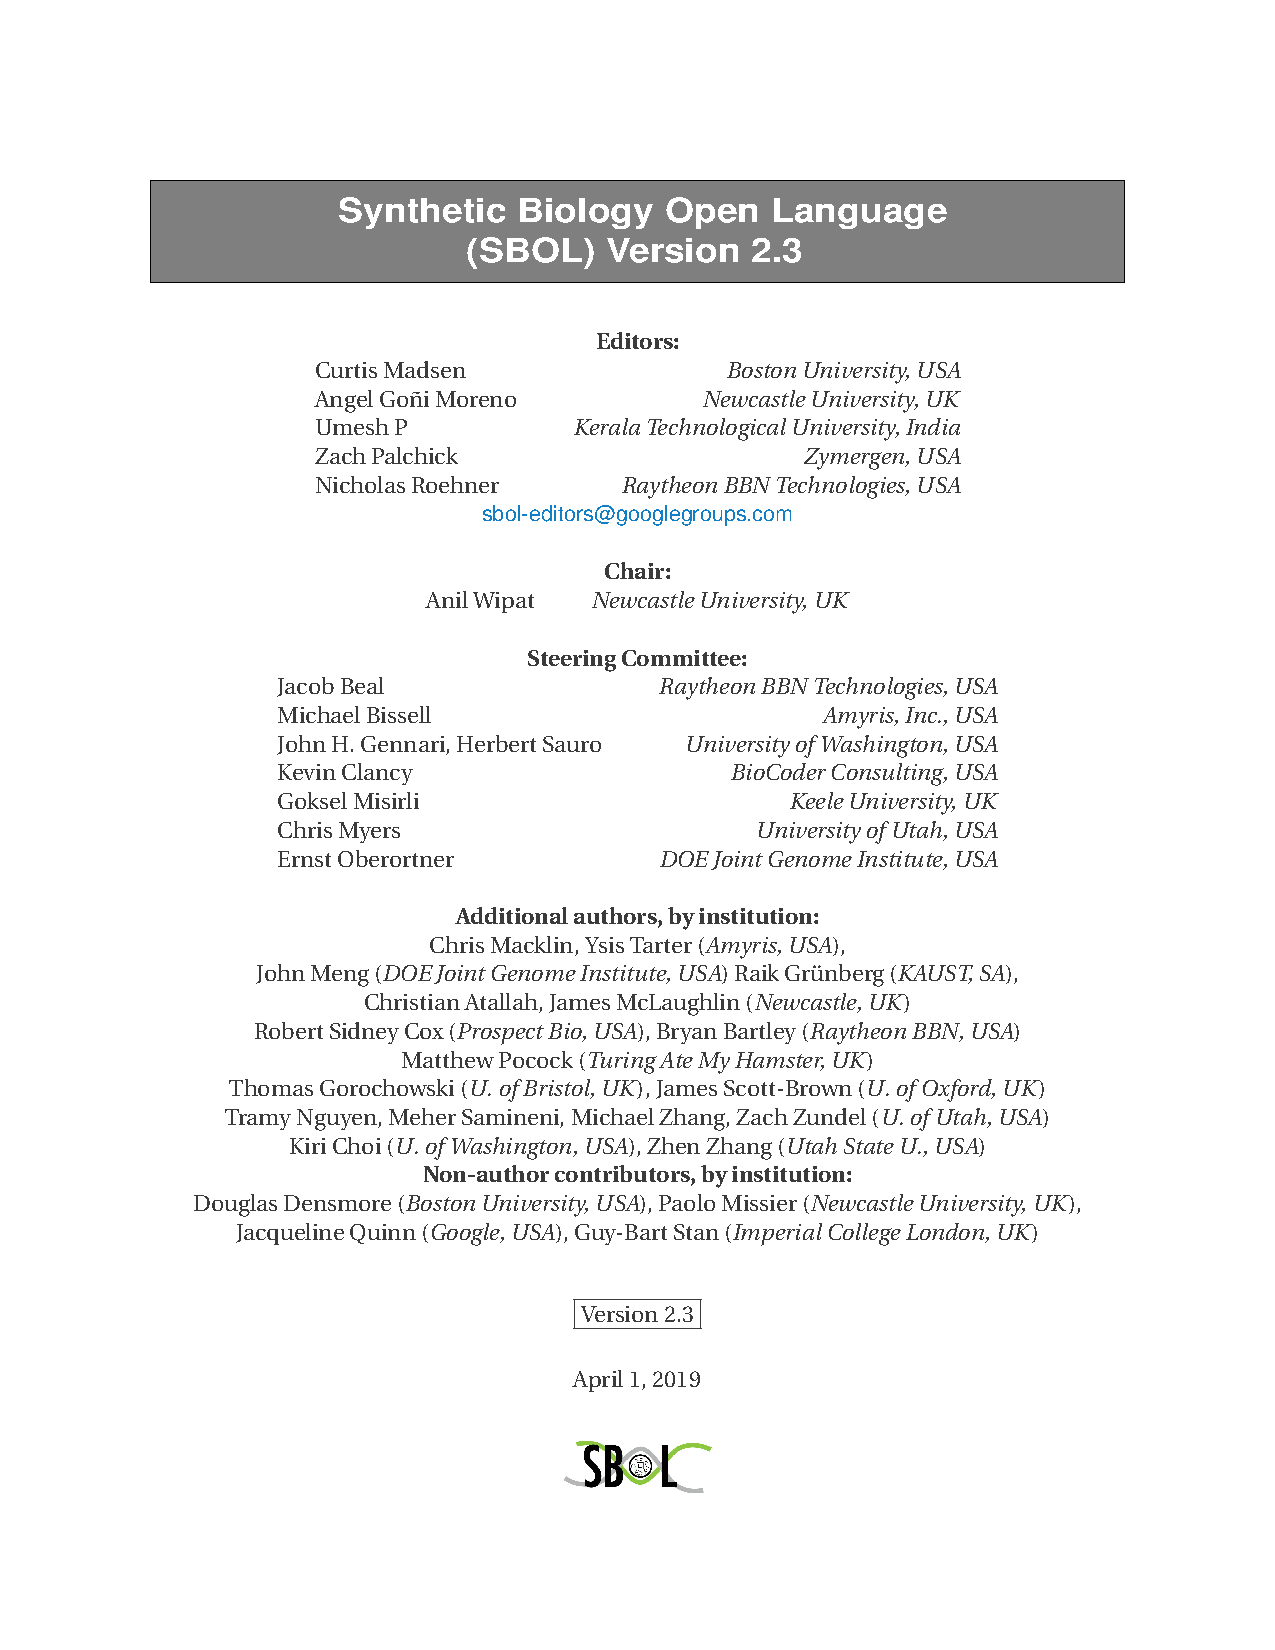
\includepdf[pages=-, offset=80 -80]{SBOL_2_3.pdf}

\end{document}
